\section{Analýza}%%%%%%%%%
\subsection{Motion capture}%%%%%%%%%
%(co je motion capture, mocap, koncepty a pojmy, vsetko, co som si o tom nastudovala, existujuce riesenia)
\noindent\acrfull{mocap} je technológia, ktorá zaznamenáva pohyby objektov, zvierat alebo ľudí v reálnom svete a prenáša tieto dáta do virtuálneho prostredia pre okamžitú alebo oneskorenú analýzu alebo prehrávanie. Táto technológia sa zrodila pri inovácií spôsobu animovania kreslených seriálov a filmov, kedy sa do procesu animovania začali komponovať aj počítače.

\subsubsection{História}%%%%%%%%%

Prvý pohyb charakteru v podobe animácie nám priniesol v roku 1911 karikaturista Zenas Winsor McCay. Pomocou viacerých kusov papieru, na ktorých boli zakreslené len jemné zmeny toho istého charakteru vytváral ilúziu pohybu, pri konštatnej rýchlosti prekladania týchto papierov. Ale vytvoriť takúto animáciu bolo veľmi časovo náročné pre animátora, keďže každá snímka musela byť individuálne nakreslená \cite{mocapFundamentals}. 

Daľší revolučný pokrok v animácií prinieslo štúdio Disney s animovaným filmom Snehulienka a sedem trpaslíkov, ktorý mal premiéru v roku 1973. Použitím nových alebo nepopulárnych technológií v tej dobe spravili veľký krok vo svete animácií. Štúdio vytvorilo viacrovinovú kameru (anglicky ,,\textit{multiplane camera}''), ktorá sníma 7 vrstiev umeleckých diel, ktoré sa prelínajú s rôznymi rýchlosťami a v rôznych vzdialenostiach od seba. To vytvára pocit hĺbky a paralaxy (zdanlivé posunutie objektu vzhľadom na pozadie pri zmene miesta pozorovateľa) \cite{multiplaneCam}. 
Taktiež štúdio Disney značne zakompononovalo pri produkcií vyššie spomínaného animovaného filmu koncept motion capture, kedy pre animované charaktery ručne prekreslovali z premietaného filmu na papier siluety ľudského pohybu. Film obsahoval nahrávku pohybov, póz a tanečných vystúpení tanečníkov alebo hercov. Tento spôsob animácie sa nazýva rotoskopia.
Táto technika kopírovania pohybu však už bola vynájdená skôr animátorom Maxom Fleischerom v roku 1915 a bola použitá v jeho animovanom seriály Out of the Inkwell. Podľa neho sa aj v ranných štádiach táto technika volala ako ,,Fleischerov proces'' a bola pre jeho tvorbu typická. No po vypršaní Fleischerovho patentu v roku 1934 mohli iní producenti a štúdia voľne využívať danú technológiu. 
Štúdio Disney sa teda chopilo príležitosti a táto metóda animovania ho priviedla k jeho sláve \cite{rotoscopeHistory}.

\begin{figure}[!htbp]
  \centering
  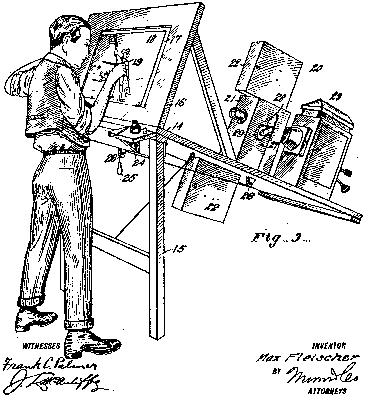
\includegraphics[width=8cm]{img/Rotoscoping-by-Max-Fleischer-Fleischer.png}
  \caption{Rotoskopia od Maxa Fleischera. (Fleischer)}
  \label{rotoscopeFig}
\end{figure}

Príchodom počítačov sa animácia zjednodušila využitím tzv. kľúčových snímkov (anglicky ,,\textit{keyframe}''), kedy sa zredukoval počet vzorkov na vytvorenie pohybu. Vytvárníkovi stačí špecifikovať začiatočnú a koncovú snímku animácie a prechod medzi týmito snímkami je automaticky generovaný \cite{mocapFundamentals}. Napriek tomu niektoré komplexné pohyby stále nebolo možné takýmto spôsobom animovať, aby si pohyb zachoval svoju prirodzenosť. 
Príkladom takého pohybu je ľudská chôdza. Človek pri jednom kroku rozpohybuje veľa častí svôjho tela a dynamika týchto častí vytvára komplexnú štruktúru celého pohybu kroku. Tieto kroky musia na seba aj prirodzene nadväzovať, aby tvorili pohyb chôdze, ktorá sa následne ešte aj komplikuje faktom, že sa nedeje na dokonalej rovine, ale v rôznorodom teréne, ktorému sa telo človeka pri chôdzi musí prispôsobovať.

V rokoch 1980 až 1983 na Univerzite Simona Frasera v biomechanických laboratóriach sa začali používať počítače na analýzu ľudského pohybu. Technika a zariadenia využívané v ich štúdiach si našli uplatnenie aj v odvetví počítačovej grafiky. Profesor kineziológie a počítačových vied na Univerzite Simona Frasera Tom Calvert využitím potenciometrov (potenciometer = premenný rezistor, ktorého odpor sa dá lineárnym pohybom alebo otočením meniť), ktoré pripojil k telu človeka, zaznamenával tak pohyb človeka a tým ovládal počítačom animovanú postavu pre choreografické a klinické výskumné účely, ako napríklad skúmanie pohybových abnormalít. Pre príklad na skúmanie ohybu kolena pripútali na každú nohu exoskeleton s potenciometrom, ktorý bol umiestnený pozdĺž každého kolena, tak aby sa ohýbal v súlade s kolenom. Takto bol vyvinutý prvý mechanický motion capture oblek na snímanie pohybov, kedy zobrali analógový výstup pohybu a previedli ho do digitálnych dát, ktoré boli spracované ich animačným systémom v počítači. No toto riešenie bolo mierne nepohodlné v rozmedzí dynamickejších pohybov.

\begin{figure}[!htbp]
  \centering
  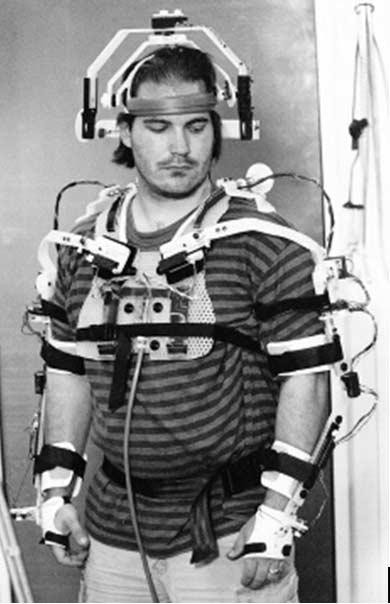
\includegraphics[width=8cm]{img/firstMechMocapSuit.jpg}
  \caption{Prvý mechanický motion capture oblek vyvinutý na Univerzite Simona Frasera}
  \label{mechMocapFig}
\end{figure}

Medzitým na Massachusettskom Technologickom Inštitúte (MIT) a Newyorskom Technologickom Inštitúte (NYIT) experimentovali s technológiou zachytávania pohybu ľudského tela s využitím optického zaznamenávacieho systému.
\acrlong{mocap} oblek je vybavený malými značkami, ktoré sú pripevnené k telu. Tieto značky sú buď ako blikajúce \acrshort{led} svetlá alebo malé reflexné body. Takto skonštruovaný oblek zachytáva séria dvoch alebo viacerých kamier. Kombináciou špeciálneho hardvéru a softvéru sa z kamerového záznamu vyberajú vyššie spomínané značky z vizuálneho poľa každej kamery a porovnávaním týchto snímkov sa kalkuluje pozícia každej značky v trojrozmernom priestore za prejdený čas záznamu.
No táto technológia je obmedzená rýchlosťou pohybu značiek (koľko pozícií značiek vie kamera zachytiť za sekunku). Toto obmedzenie má za následok rozlíšenie kamier, hlavne ich schopnosť rozoznať značky, ktoré sú blízko seba. Prvotné systémy vedeli zaznamenávať len zopár značiek naraz. Moderné systémy zvládnu spracovávať niekoľko desiatok značiek naraz. Tento problém sa vie redukovať nasadením viac sledovacích kamier, ale aj pri takomto riešení aj v moderných systémoch je potrebný manuálny post-processing záznamov, aby sa poupravili alebo obnovili trajektórie značiek, ktoré sa stratili z výhľadu kamery. Čiže pri tomto type technológie treba nájsť rovnováhu, lebo dá sa vyhnúť manuálnemu post-processingu, keď sa zainvestuje do viacero kamier alebo do kamery s kvalitnejším záznamom (vyšším rozlíšením). To nám taktiež vie zvýšiť aj zorné pole záznamu a teda aj rozsah pohybov, ktoré je možné natočiť. Aj s jednou kamerou pri dostatočnom priblížení vieme odstrániť problém stratených značiek, ale to nám obmedzuje rozsah pohybov, lebo zmenšíme zorné pole kamery. A kvôli všetkým týmto problematickým riešeniam optimalizácie procesovania záznamu aj v dnešnej dobe sa pri optickom type motion capture oblekov spoliehajú na post-procesing postupy, kvôli anlýze, sprocesovaní a dolaďovaní dát predtým ako sa aplikujú na animovanú postavu.
Tento typ motion capture systémov sa aj skomercializoval v odvetví počitačovej grafiky (napr. systémy Op-Eye alebo SelSpot).

V nasledujúcich rokoch prichádzali rôzne experimenty v oblasti motion capture systémov. 

Napríklad prvé animovanie tváre ešte aj v reálnom čase bolo poňaté ako bábkoherectvo, kedy na ovládanie významných častí tváre, ktoré v určitých pozíciach predstavujú ľudské výrazy, používali špeciálne upravený ovládač, ktorý ovládal bábkoherec. On mal pod kontorlou pohyby úst, očí, výrazov a polohu hlavy. Tento systém bol vyvinutý firmou deGraf/Wahrman. Bol zostrojený digitálnym animátorom Michaelom Wahrmanom a bývalým riaditeľom digitálnej produkcie Bradom deGrafom v roku 1987. V roku 1988 stvorili ,,Mike the Talking Head'' (slovensky ,,Mike, Rozprávajúca Hlava'') pre firmu Silicon Graphics, ktorý bol predstavený na živom vystúpení pre filmový a video festival SIGGRAPH.

Tento systém sa za pomoci firmy Pacific Data Images ešte vylepšil a vznikol Waldo C. Graphic. Toho používali ako digitálne renderovanú bábku v reálnej bábkohre, ktorá bola vysielaná v televízií. Taktiež rovnaká firma postupne vyvinula pomerne ľahký exoskeleton na záznam pohybov pre hornú časť tela a vedeli v reálnom čase zaznamenávať do ich predstavenia aj iné charaktery ako bábky. Využívali v tomto prípade potenciometre, ale toto riešenie nebolo ideálne kvôli zvuku, ktorý vydávala elektronika a taktiež exoskeleton bol stále mierna záťaž na herca.

V roku 1992 firma SimGraphics predstavila zaznamenávací systém, tzv. ,,face waldo''. Používala už menšie mechanické senzory pripevnené k brade, perám, lícam a obočiu a elektro-magnetické senzory na podpornej helme. Tento systém už taktiež vedel zaznamenávať v reálnom čase \cite{mocapHistory}.

Neskôr sa rôzne typy týchto systémov spájali a značne urýchlovali proces animovania alebo vedeli animovať väčšie časti charakterov v lepšom rozlíšení alebo viac charakterov naraz. Taktiež redukovali počet aktérov pri animovaní jedného charakteru.

Rôzne prístupy pri vývoji mocap systémov nám ich rozdelilo na rôzne typy ako akustické, mechanické, optické a magnetické \cite{mocapFundamentals}.

Dnes mocap má široké využitie v rôznych odvetviach ako je zábavný priemysel (filmy, animácie, počítačové hry), ale aj v zdravotníctve, športe a armáde. Vie ponúknuť veľmi rýchle, efektívne, finančne prijateľné spracovanie pohybov tela a/alebo tváre pre vytvorenie animácií rôznych charakterov. V ďaľšej sekcii (\ref{ssec:hw}) si priblížime nami použitý oblek \acrfull{pn3}.

\section{Softvérové a hardvérové prostriedky}%%%%%%%%%%%%%%%%%%%%%%
\subsection{Softvér}%%%%%%%%%%%%%%%%%%%%%%%%%%%%%%%%%%%%%%%%%%%%%%%

\subsection{Hardvér}%%%%%%%%%%%%%%%%%%%%%%%%%%%%%%%%%%%%%%%%%%%%%%%
\label{ssec:hw}

\section{Recitácia}

Citujem všetky zdroje v \textbf{bibliography.bib}, \cite{t00, t01, t02, t03, kniha, kniha2, kniha3, small, big, cs, koll, kap, tug, knuth, zbornik, prispevok}. \newline Good luck.
\section{Možnosti anonymizácie}
\noindent Anonymizácia znamená zmena alebo úprava údajov tak, aby sa podľa nich nedala jednoznačne určiť osoba, ktorej tieto údaje patria \cite{t01}. Existuje niekoľko spôsobov, ktorými môžeme dosiahnuť rôznu úroveň anonymizácie na internete: od mazania cookies súborov po ukončení prehliadania webových stránok až po používanie operačných systémov, ktoré sú na anonymite založené; od bezplatných možností až po komerčné verzie.  
\newline Nasleduje priblíženie niektorých možnosti anonymizácie.

\subsection{Súkromné prehliadanie}
\noindent Najpoužívanejšie internetové prehliadače súčasnosti majú v sebe zabudovanú funkcionalitu, ktorá dokáže čiastočne anonymizovať prístup na internet. Táto funkcionalita blokuje ukladanie navštívených stránok do histórie a nezaznamenáva súbory, ktoré sa stiahnu z~internetu. \acrshort{sw} a \acrlong{hw} sú skratky.

\begin{table}[!htbp]
\caption{Moduly a ich funkcie pri anonymizácii}
\label{modulyVlastnosti}
\begin{center}
\begin{tabular}{p{4cm}|c|c|c|c|c|c|c|c|c|c|c|c|c|c|c}
& \multicolumn{14}{c}%
	 {\textbf{Funkcia}}\\ \hline
&&&& & &\multicolumn{8}{c}%
	 {Modifikácia}\\ 
\textbf{Modul} &\begin{sideways} zobrazenie hlavičky \end{sideways} &\begin{sideways} blokovanie skriptov \end{sideways} &\begin{sideways} zmena IP \end{sideways} & \begin{sideways} zmena lokalizácie \end{sideways} & \begin{sideways} zmazanie/blokovanie cookies \end{sideways} & \begin{sideways} blokovanie trackerov \end{sideways}  & \begin{sideways} popis \end{sideways} & \begin{sideways}používateľský agent\end{sideways} & \begin{sideways} kódové označenie prehliadača \end{sideways} & \begin{sideways} názov prehliadača \end{sideways} & \begin{sideways} verzia prehliadača \end{sideways} & \begin{sideways} platforma \end{sideways} & \begin{sideways} výrobca prehliadača \end{sideways} & \begin{sideways} označenie výrobcu prehliadača \end{sideways} \\ \hline
User agent switcher & & & & & &  & X & X & X & X & X & X & X & X  \\ \hline
Ghostery &  && & & X & X &  &  & & & & & & \\  \hline
Better privacy && &  & & X &  &  &  & & & & & & \\  \hline
Anonymox &  && X & X & X &  & X & X & & & & & & \\  \hline
Modify headers & & &  &  & X &  &  & X &  &  &  & & &  \\  \hline
Request policy & & &  &  & & X  &  &  &  &  &  & & &   \\  \hline
Live HTTP headers & X& &  &  & &  &  &  &  &  &  & & &   \\  \hline
User agent awitcher & & &  &  & &  & X & X &  &  &  & & &   \\  \hline
Header hacker & & &  &  & &  & X & X & X & X & X & X & X & X    \\  \hline
Mod header & & &  &  & &  & X & X & X & X & X & X & X & X    \\  \hline
Script no & &X &  &  & &  &  &  &  &  &  &  &  &     \\  \hline
No script & &X &  &  & &  &  &  &  &  &  &  &  &     \\  \hline
Proxify it & & &X  & X & &  &  &  &  &  &  &  &  &     \\  \hline
I'm not here & & &  & X & &  &  &  &  &  &  &  &  &     \\  \hline
Get edition & &X &X &X &X&X &  &  &  &  &  &  &  &     \\  \hline
Anonymous browsing toolbar & & & X & X & &  &  &  &  &  &  &  &  &     \\  \hline
Easy hide your IP and surf & & & X & X& &  &  & X & X & X & X &  &  &     \\  \hline
\end{tabular}
\end{center}
\end{table}

\subsection{Anonymná sieť}
\noindent Anonymná sieť je sieť serverov, medzi ktorými dáta prechádzajú šifrované. V anonymných sieťach dáta prechádzajú z počítača používateľa, odkiaľ bola požiadavka poslaná, cez viaceré proxy smerovače, z ktorých každý správu doplní o smerovanie a zašifruje vlastným kľúčom. Cesta od ...


\subsection{Funkcionalita}
\noindent  Rozšírenie tiež okrem splnenia špecifikácie malo pre prehľadnosť a overenie funkčnosti zobrazovať údaje, ktoré boli na server odoslané. Zoznam údajov odoslaných na server, sa mal ukladať do krátkodobej histórie, aby nemal používateľ k dispozícií len najnovšie údaje, ale aj údaje odoslané v nejakom časovom období. Nejaky listing z priloh \ref{lst:sublime}.

\subsubsection{Funkcionalita2}
\noindent Samozrejmosťou bolo nastavenie zapnutia rozšírenia pri štarte, prípadne interval zmeny odosielaných údajov.

\subsection{Vzhľad}
\noindent Dôležitou požiadavkou kladenou na rozšírenie bolo príjemné používateľské rozhranie. Z~tohto dôvodu malo rozšírenie obsahovať zoznam modifikovaných vlastností a tlačidlo pre prístup k nastaveniam rozšírenia v jednoduchej a praktickej forme. Predpokladaný vzhľad je zobrazený na obrázku č. \ref{vzhladobr}.
\begin{figure}[!htbp]
  \centering
  \includegraphics[width=8cm]{img/vzhlad.png}
  \caption{Predpokladaný vzhľad rozšírenia.}
  \label{vzhladobr}
\end{figure}	 
\noindent Dôležitou požiadavkou kladenou na rozšírenie bolo príjemné používateľské rozhranie.\cite{t00} Z~tohto dôvodu malo rozšírenie obsahovať zoznam modifikovaných vlastností a tlačidlo pre prístup k nastaveniam rozšírenia v jednoduchej a praktickej forme. Predpokladaný vzhľad je zobrazený na obrázku č. \ref{vzhladobr}.

\begin{algorithm}
\scriptsize
\begin{algorithmic}
 \STATE <text>
 \IF{<condition>} \STATE {<text>} \ELSE \STATE{<text>} \ENDIF
 \IF{<condition>} \STATE {<text>} \ELSIF{<condition>} \STATE{<text>} \ENDIF
 \FOR{<condition>} \STATE {<text>} \ENDFOR
 \FOR{<condition> \TO <condition> } \STATE {<text>} \ENDFOR
 \FORALL{<condition>} \STATE{<text>} \ENDFOR
 \WHILE{<condition>} \STATE{<text>} \ENDWHILE
 \REPEAT \STATE{<text>} \UNTIL{<condition>}
 \LOOP \STATE{<text>} \ENDLOOP
 \REQUIRE <text>
 \ENSURE <text>
 \RETURN <text>
 \PRINT <text>
 \COMMENT{<text>}
 \AND, \OR, \XOR, \NOT, \TO, \TRUE, \FALSE
\end{algorithmic}
\caption{Ukážka príkazov pre algorithmic}  
\label{alg:preview}  
\end{algorithm}

\begin{lstlisting}[
  caption={Ukážka algoritmu},
  label={lst:main-c},
  language=c
]
/* Hello World program */

#include<stdio.h>

struct cpu_info {
    long unsigned utime, ntime, stime, itime;
    long unsigned iowtime, irqtime, sirqtime;
};

main()
{
    printf("Hello World");
}
\end{lstlisting}
